%% Figure 4: a simulate-infer-evaluate loop expressed in the public API.
%%
%% Each labelled step names the call that performs it, so the figure can be
%% checked against examples/sim_recovery.py and against the listings in
%% sections/examples.tex.

\documentclass[border=6pt]{standalone}
\usepackage{tikz}
\usepackage{amssymb}
\usetikzlibrary{arrows.meta,positioning,fit,backgrounds,calc}
\usepackage{xcolor}
\providecommand{\code}[1]{\texttt{#1}}
% The API call that performs a step, shown under the step name.
\newcommand{\apicall}[1]{{\ttfamily\scriptsize\color{black!65}#1}}
\begin{document}
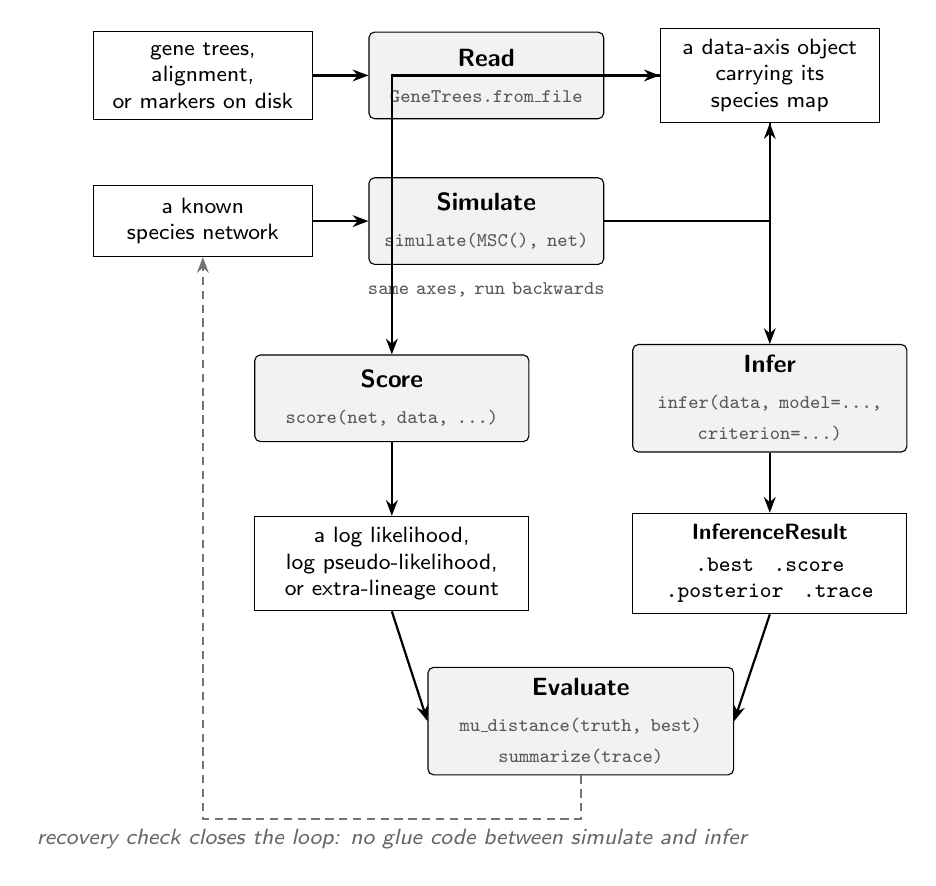
\begin{tikzpicture}[
  font=\sffamily\small,
  stage/.style={
    draw, rounded corners=2pt, align=center, fill=black!5,
    text width=27mm, minimum height=11mm, inner sep=4pt
  },
  artefact/.style={
    draw, align=center, fill=white, text width=25mm,
    minimum height=9mm, inner sep=4pt, font=\sffamily\footnotesize
  },
  call/.style={font=\ttfamily\scriptsize, text=black!65, align=center},
  flow/.style={-{Stealth[length=2mm]}, thick},
  back/.style={-{Stealth[length=2mm]}, thick, densely dashed, black!55},
]

% ---- row 1: getting data in --------------------------------------------
\node[artefact] (files) at (0, 2.2)
  {gene trees, alignment,\\ or markers on disk};
\node[stage]    (read)  at (3.6, 2.2) {\textbf{Read}\\[2pt]
  \apicall{GeneTrees.from\_file}};
\node[artefact] (dataobj) at (7.2, 2.2)
  {a data-axis object\\ carrying its\\ species map};

\draw[flow] (files) -- (read);
\draw[flow] (read)  -- (dataobj);

% simulation as the alternative source of data
\node[stage] (sim) at (3.6, 0.35) {\textbf{Simulate}\\[2pt]
  \apicall{simulate(MSC(), net)}};
\node[artefact] (truth) at (0, 0.35) {a known\\ species network};
\draw[flow] (truth) -- (sim);
\draw[flow] (sim.east) -| (dataobj.south);

\node[call, below=1mm of sim, text width=34mm]
  {same axes, run backwards};

% ---- row 2: the two verbs ----------------------------------------------
\node[stage, text width=32mm] (infer) at (7.2, -1.9)
  {\textbf{Infer}\\[2pt]
   \apicall{infer(data, model=...,}\\ \apicall{criterion=...)}};
\node[stage, text width=32mm] (score) at (2.4, -1.9)
  {\textbf{Score}\\[2pt]
   \apicall{score(net, data, ...)}};

\draw[flow] (dataobj) -- (infer);
\draw[flow] (dataobj.west) -| (score.north);

% ---- row 3: results ----------------------------------------------------
\node[artefact, text width=32mm] (result) at (7.2, -4.0)
  {\textbf{InferenceResult}\\[2pt]
   \code{.best} \, \code{.score}\\
   \code{.posterior} \, \code{.trace}};
\draw[flow] (infer) -- (result);

\node[artefact, text width=32mm] (number) at (2.4, -4.0)
  {a log likelihood,\\ log pseudo-likelihood,\\ or extra-lineage count};
\draw[flow] (score) -- (number);

% ---- row 4: evaluation -------------------------------------------------
\node[stage, text width=36mm] (eval) at (4.8, -6.0)
  {\textbf{Evaluate}\\[2pt]
   \apicall{mu\_distance(truth, best)}\\
   \apicall{summarize(trace)}};
\draw[flow] (result.south) -- (eval.east);
\draw[flow] (number.south) -- (eval.west);

\draw[back] (eval.south) -- ++(0, -0.55)
  -| node[pos=0.25, below, font=\sffamily\footnotesize\itshape, text=black!60]
     {recovery check closes the loop: no glue code between simulate and infer}
  (truth.south);

\end{tikzpicture}
\end{document}
